%\documentclass{report}
\documentclass[11pt,a4paper,notitlepage]{article}
\usepackage[utf8]{inputenc}
\usepackage{titling}
\usepackage{hyperref}

\title{Symbolic execution of adaptive side-channel attacks}
\author{Emilie L. Thonsgaard \and Irfansha Shaik}
\date{May 2020}

\usepackage{natbib}
\usepackage{graphicx}
\usepackage{amsmath}

\begin{document}
\begin{titlingpage}
    \maketitle
    \begin{abstract}
        In this report we review the subject of side-channel attacks and how symbolic execution is used in this context. We describe the concept of side-channel attacks and use the technology Klee to model it. Our program models a $k$-step attack. We investigate the program though experiments and evaluate the data and limitations of our program.
    \end{abstract}
\end{titlingpage}

\tableofcontents
\newpage
\setcounter{section}{-1}


\section{Todos for IS}
\label{sec:todosforis}

\begin{enumerate}
  \item Running the script for larger domain size and $k$-step attack.
  \item Added system details (specifications) as part of experimentation section.
\end{enumerate}

\newpage

\section{Introduction}
\label{cha:introduction}

Security is a crucial part of everyday aspects in the age of information.
While a lot of effort is being put into developing secure systems, some attacks can easily overcome most secure systems.
Side-channel attacks are one such type of attacks. The core is to \emph{listen} to the system from distance (often without the knowledge of data owner) and retrieve the sensitive information under the hood.

One of the current efforts to tackle side-channel attacks is to use symbolic execution techniques and quantify the information leakage (and finally avoid/minimize it).
We consider the research done by Quoc-Sang Phan et al., \cite{phan2017synthesis} regarding the synthesis of adaptive side-channel attacks.

In the following subsections, we first summarize the discussion on side-channel attacks and their synthesis as described by Quoc-Sang Phan et al. In section \ref{sec:researchquestions} we discuss the main research questions we consider.
Further in the section \ref{sec:experimentationanddesign}, we provide our modelling of the problem, experimental set-up as well as data analysis.
Finally in the section \ref{sec:futurework}, we conclude our observation and discuss possible future work in this direction.
\subsection{Side channel attacks}
\label{sec:sidechannelattacks}

Side-channel attacks are a general type of attack. The idea is that an adversary exploits non-functional aspects of a program. This can be various aspects, such as execution time, network traffic or memory. The topic of side-channel attacks is a prerequisite and the basis that supports understanding of symbolic execution. In our case we are considering adaptive side-channel attacks. These are a subgroup of attacks. The addition of calling a side-channel attack adaptive is that the attack spans over multiple runs. At each of these runs the adversary will choose a value for so-called low input. In this context low input means the public input. The adversary will make a choice by considering all previous runs. This attributes to the attacker's knowledge. One can think of this adversary concretely as though he is gradually recovering a secret value. In this case a value that is a constant between all the runs, such as a secret key in cryptography. 

\subsubsection{Formal definition}

We are going to define side-channel attacks. First we define a program $P(H,L)$. $P$ is a deterministic program. $H$ is the high input, which is defined as the secret input in this context. $L$ is the low input, which is defined as the public input in this context. To define the attack we make two assumptions. Firstly, the attacker can make \textit{one} observation in each run and there are no errors in his measurements. Secondly, the attackers knows the details of how the program $P$ is implemented. The idea is that the attacker can not make an observation to retrieve the entire secret data in just one round. The point is to make the attack adaptive with multiple runs and gradually learn from each try. By changing his choice of low input, he should learn different information about the secret data in each run. 

\subsubsection{Attacker model}

An attacker model strives to specify how the attacker is defined in regards to access and participation in the communication. Here the attacker is defined as a partial function $A$. Since he has to make choices based on previous observations, he takes the set of prior observations as input. $A$ returns the low value $l$ that he will use in the next attack run. 
\\An attack is defined as a $k$-step process. \cite{phan2017synthesis} models the interaction between the attacker $A$ and the program $P$ as a system $S = (A,P,k,cost(\cdot))$. $A$ is the attacker, $P$ is the program, $k$ is the step and $cost(\cdot)$ determines the side-channel observations for the execution. In $S$, $A$ chooses $l$ values for multiple program runs to determine a secret $h$. 

\subsubsection{Attacker's knowledge}

After full execution of $k$ steps, the attacker makes $k$ observations $o_1,o_2,...,o_k$ after choosing $l$ values $l_1,l_2,...,l_k$. We talk about the secret as having an initial domain $D$. What the attacker exactly learns in each step is that giving $l_i$ 

\subsection{Symbolic execution}
\label{sec:symbolicexecution}
This section is written on the basis of \cite{phan2017synthesis} and \cite{malacaria2018symbolic}.
\\\\
Symbolic analysis is concerned with techniques that can e.g. detect vulnerabilities due to side-channel attacks. Symbolic execution is a program analysis technique. It executes a program on symbolic inputs. The symbolic inputs represent concrete inputs. The analysis results in symbolic paths. Each path has a path condition. A path condition is a conjunction of constraints, and these are from the set of symbolic inputs characterizing the concrete inputs following that path. The solution to dealing with loops and recursion is to put a bound on the depth of the paths.  

\subsubsection{Symbolic attacker model}
There are a few alterations from the original attacker model. In this case we call it a system defined as $S_{sym}(P,k,cost(\cdot))$. The secret $h$ is modelled using a symbolic variable. The other difference is that low values $l$ are also modelled using a fresh symbolic variable, since we do not know the maximal leakage low value in advance.
\\The symbolic execution $S_{sym}$ results in a set of symbolic paths corresponding to the $k$ steps. The resulting paths represent all the potential adaptive attacks up to $k$ runs. 
\\The outcome of symbolically executing $S_{sym}$ is the beforementioned paths. These can be organized into a tree. In the tree, nodes are the attacker moves, which means the choice of low values based on observations. On the path there are path conditions computed for different observations. The leaves are path constraints. They represent the attacker's knowledge after $k$ steps. 

\subsubsection{Synthesizing attacks}
It is possible to use greedy heuristics to save computation power. They can be used for generating the attack such that you explore a portion of the symbolic attack model in each step. Some of these heuristics are based on two measurements that are possible to calculate. They are \textit{channel capacity} and \textit{Shannon entropy}. They can be used to reason about sequences of observations in the system. 
\\Channel capacity \cite{smithQIF} is based on a theorem that says the leakage for a program in bits is less than or equal to log of the possible distinct observations an attacker can make. 
\\Shannon entropy is a result that gives a measurement of the amount of leakage of the side-channel. It takes into account the observation gain (bits learned) of the secret value after an observation. Assume we have a sequence of observations $o_i^k = \langle o_1,o_2,...,o_k \rangle$, then $p(o_i^k)$ is the probability of observing $o_i^k$. Shannon entropy is defined as 
\begin{align*}
    \mathcal{H}^k(P) = -\sum_{o_i^k} p(o_i^k) log_2(p(o_i^k))
\end{align*}
The best attacker picks low values that result in the highest leakage.

\section{Research questions}
\label{sec:researchquestions}

Symbolic execution/analysis does result in optimal attack synthesis among other advantages, it is due to all possible paths are modelled into constraints and then analysed.
However, the obvious challenge is that the state space increases exponentially.
Different tools employ different techniques to overcome this well know challenge, now the question here is \emph{What does Klee do differently?}
In the literature XXX add paper, Symbolic Path Finder is a java based symbolic tool was used to analyze the adaptive side channel attack and quantify information leakage.
The SPF implementation of this problem timeout for larger domains and k (XXX add more accurate data) and they employed heuristics to explore some set states to achieve better scalability (to some extent).

In this project, we want to investigate if \texttt{Klee} employ any specific techniques for scalability.
There are several heuristics for exploring the search space and solver chains that can be used.

Investigating solvers chains is essential for symbolic execution, as the most of the time spent is in solver execution.
In this project, for the adaptive side channel attack we investigate the impact of various solvers provided in \texttt{Klee}.

\section{Experimentation setup and Analysis}
\label{sec:experimentationanddesign}

To invesigate the scalability of adaptive side channel attacks in \texttt{Klee}, we first model a side channel attack and investigate the adaptive $k$-step attack in \texttt{Klee}.

\subsection{Modelling the adaptive symbolic side channel attack}
\label{subsec:modellingsscattack}

We consider a simple side channel attack via symbolic execution.
Consider the code snippet provided below (source code available in \href{https://github.com/irfansha/LBS_projects.git}{github}):
\begin{verbatim}
int vulnerable_code(int public_input) {

if (secret >= public_input) { return 1; } // Cost is 1
else { return 2; } // Cost is 2

}
\end{verbatim}

As in any side channel attack, we need difference in some measurement (for example time) here we simply provide the cost as integer
for comparision between different paths.

Now the idea is to apply $k$-step attack, such that we extract some information on secret key.
For example, let $\{1 \dots 6\}$ be the domain of the secret (which we assume to know) and suppose we apply a $2$-step attack.
Here, we choose two public inputs such that we slice the domain such that we retrive the secret key depending on the cost measurement.
Given enough $k$, it is possible to retreive the secret key completely however it is not practical as search tree size grows exponentially.
However, if we simply choose $k$ independent public inputs then narrowing down to the secret is very hard.
On the other hand, choosing public inputs based on previous cost observations make it very easy.
For example, for the above example if we choose ${5,6}$ where the costs observed are ${1,2}$ respectively thus the domain is restricted to ${6}$ via ${5,6}$. It is clear that adaptive attacks are very powerful.

The challenge here is to model all possible paths of publich inputs and secret, thus we make them symbolic.
The following is syntax for making variables symbolic in \texttt{Klee}
\begin{verbatim}
// Making the secret symbolic:
klee_make_symbolic(&secret,sizeof(int),"secret");

// Making the public inputs symbolic:
klee_make_symbolic(public_inputs,k * sizeof(int),"public inputs");
\end{verbatim}

Usually symbolic execution is used for synthesis of best side channel attack (we discuss further in outlook section XXX), however here we will only investigate the scalability of \texttt{Klee}.
But it is important to note that in symbolic analysis, which \emph{encodes} all paths in terms of path conditions, it is possible to identify the leakage and thus synthesize best side channel attack.

Now the major challenge is to simulate adaptive attack, in \texttt{Klee} there is no explicit way to specify the bounds of each symbolic variable (that we aware of).
As discussed in the above example the domain of the secret reduces by the pervious cost observations, we model this by left and right bounds (lb, rb) which are updated through out the execution.
Here is the snippet of code that narrows down the secret domain via left and right bounds:
\begin{verbatim}
// Iterate and run `vulnerable function'
for [each k] {
  int cost = vulnerable_function(public_inputs[step]);

  //Here we update the domain boundaries secret input
  if (cost == 1) { rb = public_inputs[step] - 1;}
  else { lb = public_inputs[step]; }

}
\end{verbatim}

Finally, we will only consider valid inputs i.e., we check if the public input is within current bounds and if it is non repeating.
While this generates some additional paths, they are only linear in the number of steps.
Using this modelling, we investigate the scalability in \texttt{Klee} and we discuss our experimental setup below.

\subsection{Software: \texttt{Klee} and our experimentation setup}
\label{subsec:softwares}

\href{https://klee.github.io/}{\texttt{Klee}} is a open source symbolic execution tool that runs on top of LLVM infrastructure.
More details are presented in paper XXX.
Generally used to analyse the coverage of code in C/C++ which is inturn compiled into LLVM. 

We use our adaptive side channel attack model, and investigate different heuristics and solvers provided by \texttt{Klee}.
Here are the list of heuristics we consider:
\begin{enumerate}
\item dfs - uses Depth First Search (DFS)
\item random-state - randomly selects a state to explore
\item random-path - uses Random Path Selection
\item Non Uniform Random Search (NURS):
  \begin{enumerate}
  \item covnew - uses Coverage-New heuristic
  \item md2u - uses Min-Dist-to-Uncovered heuristic
  \item depth - uses $2^d$ ($d$ is depth) heuristic
  \item icnt - uses Instr-Count heuristic
  \item cpicnt - uses CallPath-Instr-Count heuristic
  \item qc- uses Query-Cost heuristic
  \end{enumerate}
\item we also consider no heuristics and all heuristics interleaved.
\end{enumerate}

A key point to remember with the different heuristics is that, they only dictate with symbolic state to expand next.
That implies, a full scale exploration of search trees will not be effected much by the heuristics.
In our experimentation we cut of the trees with certain $k$ so heuristics might play a role here (or not).

Here are the solvers we consider:
\begin{enumerate}
\item STP
\item Z3
\item Counter example  caching solver
\item Independence solver
\end{enumerate}

It is well known that, in symbolic execution the major time spent is in solver computations, thus it is crucial to investigate the scalability of solvers that are available in \texttt{Klee}
For our experiments, we use a computer with following specification:
\begin{verbatim}
Architecture: x86_64
CPU(s):       4
Model name:   Intel(R) Core(TM) i5-5200U CPU @ 2.20GHZ
BogoMIPS:     4389.72
\end{verbatim}

The source code for our symbolic adaptive side channel attack is available here XXX.
The script we use for running different heuristics and solvers are also available in the same repository.

\subsection{Data and analysis}
\label{subsec:dataandanalysis}

Following the experimentation set-up, we have generated data for various heuristics and solvers (raw data is available here XXX).
For scalability, we are consider two parameters, total time and solver time for increasing domain sizes and $k$ steps.

The figures \ref{fig:basic_heur_tt} and \ref{fig:basic_heur_st} illustrate the total and solver time for basic heuristics.XXX
Similarly, the figures \ref{fig:nonuni_heur_tt} and \ref{fig:nonuni_heur_st} show the variation for non-uniform random heuristics.

\begin{figure}[h]
\centering
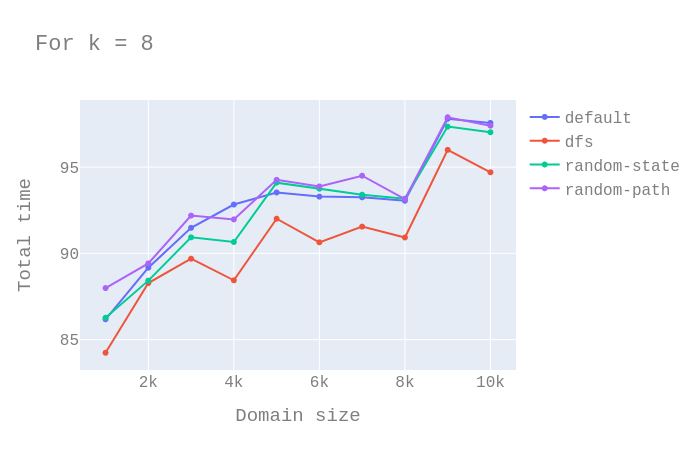
\includegraphics[width=10cm]{k_8_tt_basic_heur.png}
\label{fig:basic_heur_tt}
\caption{Total time with basic heuristics}
\centering
\end{figure}

\begin{figure}[h]
\centering
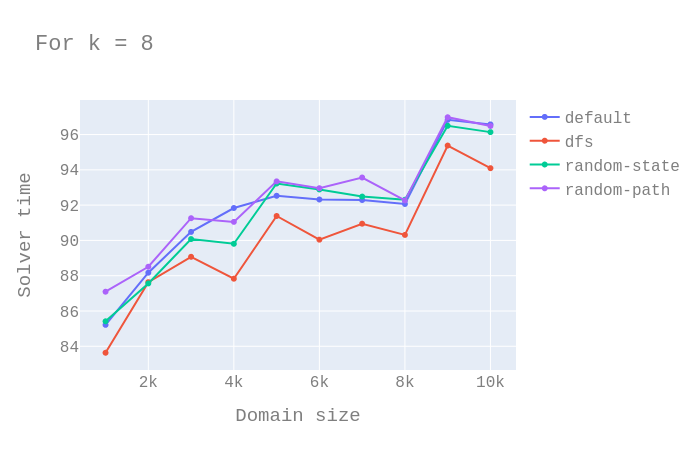
\includegraphics[width=10cm]{k_8_st_basic_heur.png}
\label{fig:basic_heur_st}
\caption{Solver time with basic heuristics}
\centering
\end{figure}

\begin{figure}[h]
\centering
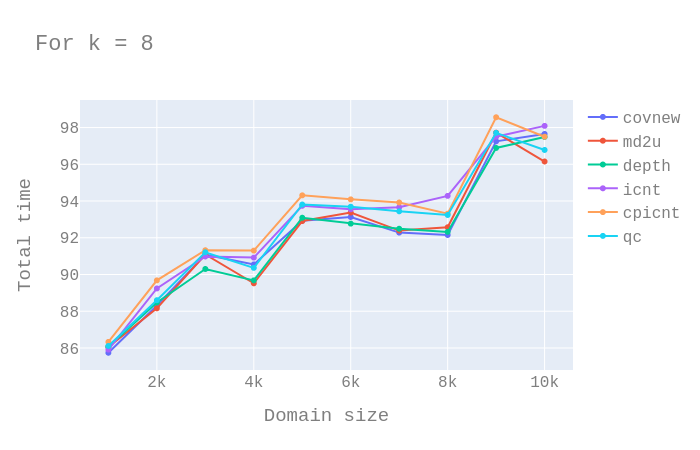
\includegraphics[width=10cm]{k_8_tt_nonuni_heur.png}
\label{fig:nonuni_heur_tt}
\caption{Total time with Non-uniform random heuristics}
\centering
\end{figure}

\begin{figure}[h]
\centering
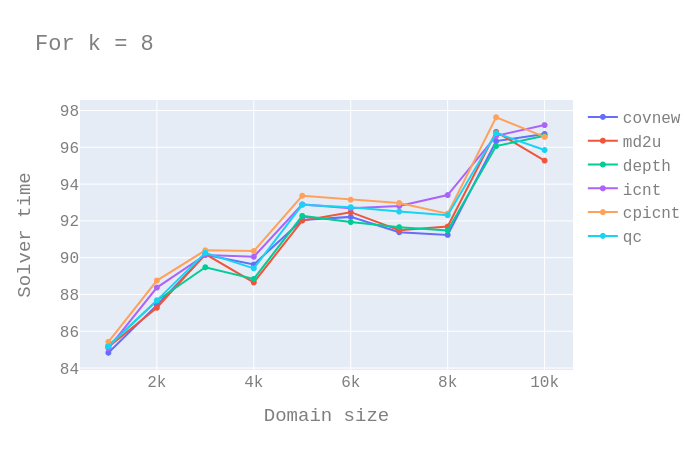
\includegraphics[width=10cm]{k_8_st_nonuni_heur.png}
\label{fig:nonuni_heur_st}
\caption{Solver time with Non-uniform random heuristics}
\centering
\end{figure}

The table \ref{fig:solvertime} provide the solver times for different solvers.
Here the total time is almost equal to the solver times(usually $97$ percentage),
so looking at solver times is sufficient enough to get a good idea.

\begin{figure}
\centering
\begin{tabular}{|c|c|c|c|c|}
\hline
\textbf{Domain size} & stp & z3 & cex & ind \\ \hline \hline
1000 & 84.908256 & 201.205725 & 86.578195 & 84.817953 \\
2000 & 88.516439 & 212.2281 & 88.266316 & 87.881535 \\
3000 & 90.361902 & 220.282183 & 90.698298 & 91.460136 \\
4000 & 90.868617 & 227.692224 & 89.768262 & 90.965436 \\
5000 & 92.249937 & 237.322899 & 93.407886 & 92.557288 \\
6000 & 91.73592 & 232.597158 & 91.774256 & 92.16203 \\
7000 & 92.14107 & 236.883911 & 92.170761 & 91.923944 \\
8000 & 91.497112 & 238.015212 & 92.022306 & 92.270304 \\
9000 & 98.2179 & 252.089498 & 96.723129 & 96.277674 \\
10000 & 96.0498 & 248.172816 & 95.971008 & 96.822 \\
\hline
\end{tabular}
\caption{Solver time spent for various solvers ($k = 8$).}
\label{fig:solvertime}
\end{figure}


From the table it is clear that, Z3 performs surprisingly worse compared to other solvers.
However the difference is not exponentially increasing but perhaps only a constant.

The following table presents the extend we were able to run for the domain size XXX and increasing $k$

XXX


\section{Conclusion and future work}
\label{sec:futurework}

Symbolic execution of adaptive side channel attack is an earlier stage of bigger problem i.e., the synthesis of optimal side channel attack.
The natural next step is to use the data produced in section XXX (instead of explicit data, a constraint solver can be used to find right values) and synthesising the public inputs with maximum information leakage.

\subsection{Initial investigation on quantifying informations leakage and \texttt{Klee} heuristics}
\label{subsec:initialinvestigationleakage}

We generated data (XXX add link) for different heuristics and investigated if new paths are observed for different heuristics.
We applied brute force search, i.e., searching through all paths of basic run data (without heuristics) and compared with various heuristics.
The observations are not so significant, we observed some paths are being explored via new heuristics but they are quite rare questioning the impact of heuristics.
However, it is important to note that we did not drive our symbolic attack towards maximizing the secret leakage.
For example, asserting if the final bounds (lb and rb) are equal can guide \texttt{Klee} towards better information leakage.
Thus, heuristics might play a bigger role in regards to synthesis of best side channel attacks and better scalability which still needs to be investigated.



\bibliographystyle{plain}
\bibliography{references}
\end{document}
